% Options for packages loaded elsewhere
\PassOptionsToPackage{unicode}{hyperref}
\PassOptionsToPackage{hyphens}{url}
%
\documentclass[
]{article}
\usepackage{amsmath,amssymb}
\usepackage{iftex}
\ifPDFTeX
  \usepackage[T1]{fontenc}
  \usepackage[utf8]{inputenc}
  \usepackage{textcomp} % provide euro and other symbols
\else % if luatex or xetex
  \usepackage{unicode-math} % this also loads fontspec
  \defaultfontfeatures{Scale=MatchLowercase}
  \defaultfontfeatures[\rmfamily]{Ligatures=TeX,Scale=1}
\fi
\usepackage{lmodern}
\ifPDFTeX\else
  % xetex/luatex font selection
\fi
% Use upquote if available, for straight quotes in verbatim environments
\IfFileExists{upquote.sty}{\usepackage{upquote}}{}
\IfFileExists{microtype.sty}{% use microtype if available
  \usepackage[]{microtype}
  \UseMicrotypeSet[protrusion]{basicmath} % disable protrusion for tt fonts
}{}
\makeatletter
\@ifundefined{KOMAClassName}{% if non-KOMA class
  \IfFileExists{parskip.sty}{%
    \usepackage{parskip}
  }{% else
    \setlength{\parindent}{0pt}
    \setlength{\parskip}{6pt plus 2pt minus 1pt}}
}{% if KOMA class
  \KOMAoptions{parskip=half}}
\makeatother
\usepackage{xcolor}
\usepackage[margin=1in]{geometry}
\usepackage{color}
\usepackage{fancyvrb}
\newcommand{\VerbBar}{|}
\newcommand{\VERB}{\Verb[commandchars=\\\{\}]}
\DefineVerbatimEnvironment{Highlighting}{Verbatim}{commandchars=\\\{\}}
% Add ',fontsize=\small' for more characters per line
\usepackage{framed}
\definecolor{shadecolor}{RGB}{248,248,248}
\newenvironment{Shaded}{\begin{snugshade}}{\end{snugshade}}
\newcommand{\AlertTok}[1]{\textcolor[rgb]{0.94,0.16,0.16}{#1}}
\newcommand{\AnnotationTok}[1]{\textcolor[rgb]{0.56,0.35,0.01}{\textbf{\textit{#1}}}}
\newcommand{\AttributeTok}[1]{\textcolor[rgb]{0.13,0.29,0.53}{#1}}
\newcommand{\BaseNTok}[1]{\textcolor[rgb]{0.00,0.00,0.81}{#1}}
\newcommand{\BuiltInTok}[1]{#1}
\newcommand{\CharTok}[1]{\textcolor[rgb]{0.31,0.60,0.02}{#1}}
\newcommand{\CommentTok}[1]{\textcolor[rgb]{0.56,0.35,0.01}{\textit{#1}}}
\newcommand{\CommentVarTok}[1]{\textcolor[rgb]{0.56,0.35,0.01}{\textbf{\textit{#1}}}}
\newcommand{\ConstantTok}[1]{\textcolor[rgb]{0.56,0.35,0.01}{#1}}
\newcommand{\ControlFlowTok}[1]{\textcolor[rgb]{0.13,0.29,0.53}{\textbf{#1}}}
\newcommand{\DataTypeTok}[1]{\textcolor[rgb]{0.13,0.29,0.53}{#1}}
\newcommand{\DecValTok}[1]{\textcolor[rgb]{0.00,0.00,0.81}{#1}}
\newcommand{\DocumentationTok}[1]{\textcolor[rgb]{0.56,0.35,0.01}{\textbf{\textit{#1}}}}
\newcommand{\ErrorTok}[1]{\textcolor[rgb]{0.64,0.00,0.00}{\textbf{#1}}}
\newcommand{\ExtensionTok}[1]{#1}
\newcommand{\FloatTok}[1]{\textcolor[rgb]{0.00,0.00,0.81}{#1}}
\newcommand{\FunctionTok}[1]{\textcolor[rgb]{0.13,0.29,0.53}{\textbf{#1}}}
\newcommand{\ImportTok}[1]{#1}
\newcommand{\InformationTok}[1]{\textcolor[rgb]{0.56,0.35,0.01}{\textbf{\textit{#1}}}}
\newcommand{\KeywordTok}[1]{\textcolor[rgb]{0.13,0.29,0.53}{\textbf{#1}}}
\newcommand{\NormalTok}[1]{#1}
\newcommand{\OperatorTok}[1]{\textcolor[rgb]{0.81,0.36,0.00}{\textbf{#1}}}
\newcommand{\OtherTok}[1]{\textcolor[rgb]{0.56,0.35,0.01}{#1}}
\newcommand{\PreprocessorTok}[1]{\textcolor[rgb]{0.56,0.35,0.01}{\textit{#1}}}
\newcommand{\RegionMarkerTok}[1]{#1}
\newcommand{\SpecialCharTok}[1]{\textcolor[rgb]{0.81,0.36,0.00}{\textbf{#1}}}
\newcommand{\SpecialStringTok}[1]{\textcolor[rgb]{0.31,0.60,0.02}{#1}}
\newcommand{\StringTok}[1]{\textcolor[rgb]{0.31,0.60,0.02}{#1}}
\newcommand{\VariableTok}[1]{\textcolor[rgb]{0.00,0.00,0.00}{#1}}
\newcommand{\VerbatimStringTok}[1]{\textcolor[rgb]{0.31,0.60,0.02}{#1}}
\newcommand{\WarningTok}[1]{\textcolor[rgb]{0.56,0.35,0.01}{\textbf{\textit{#1}}}}
\usepackage{longtable,booktabs,array}
\usepackage{calc} % for calculating minipage widths
% Correct order of tables after \paragraph or \subparagraph
\usepackage{etoolbox}
\makeatletter
\patchcmd\longtable{\par}{\if@noskipsec\mbox{}\fi\par}{}{}
\makeatother
% Allow footnotes in longtable head/foot
\IfFileExists{footnotehyper.sty}{\usepackage{footnotehyper}}{\usepackage{footnote}}
\makesavenoteenv{longtable}
\usepackage{graphicx}
\makeatletter
\def\maxwidth{\ifdim\Gin@nat@width>\linewidth\linewidth\else\Gin@nat@width\fi}
\def\maxheight{\ifdim\Gin@nat@height>\textheight\textheight\else\Gin@nat@height\fi}
\makeatother
% Scale images if necessary, so that they will not overflow the page
% margins by default, and it is still possible to overwrite the defaults
% using explicit options in \includegraphics[width, height, ...]{}
\setkeys{Gin}{width=\maxwidth,height=\maxheight,keepaspectratio}
% Set default figure placement to htbp
\makeatletter
\def\fps@figure{htbp}
\makeatother
\setlength{\emergencystretch}{3em} % prevent overfull lines
\providecommand{\tightlist}{%
  \setlength{\itemsep}{0pt}\setlength{\parskip}{0pt}}
\setcounter{secnumdepth}{-\maxdimen} % remove section numbering
\usepackage{pdfpages}
\ifLuaTeX
  \usepackage{selnolig}  % disable illegal ligatures
\fi
\IfFileExists{bookmark.sty}{\usepackage{bookmark}}{\usepackage{hyperref}}
\IfFileExists{xurl.sty}{\usepackage{xurl}}{} % add URL line breaks if available
\urlstyle{same}
\hypersetup{
  pdftitle={Day8 exercise solutions},
  pdfauthor={Ali Movasati},
  hidelinks,
  pdfcreator={LaTeX via pandoc}}

\title{Day8 exercise solutions}
\author{Ali Movasati}
\date{Oct.~4th, 2024}

\begin{document}
\maketitle

\begin{Shaded}
\begin{Highlighting}[]
\CommentTok{\# Set global code chunk options}
\NormalTok{knitr}\SpecialCharTok{::}\NormalTok{opts\_chunk}\SpecialCharTok{$}\FunctionTok{set}\NormalTok{(}\AttributeTok{warning =} \ConstantTok{FALSE}\NormalTok{)}
\end{Highlighting}
\end{Shaded}

\begin{Shaded}
\begin{Highlighting}[]
\CommentTok{\# load required libraries}
\FunctionTok{library}\NormalTok{(}\StringTok{"skimr"}\NormalTok{)}
\FunctionTok{library}\NormalTok{(}\StringTok{"dplyr"}\NormalTok{)}
\FunctionTok{library}\NormalTok{(}\StringTok{"magrittr"}\NormalTok{)}
\FunctionTok{library}\NormalTok{(}\StringTok{"ggplot2"}\NormalTok{)}

\CommentTok{\# define functions}
\StringTok{\textasciigrave{}}\AttributeTok{\%notin\%}\StringTok{\textasciigrave{}} \OtherTok{\textless{}{-}} \FunctionTok{Negate}\NormalTok{(}\StringTok{\textasciigrave{}}\AttributeTok{\%in\%}\StringTok{\textasciigrave{}}\NormalTok{)}
\end{Highlighting}
\end{Shaded}

\section{Problem 1}\label{problem-1}

\begin{Shaded}
\begin{Highlighting}[]
\FunctionTok{data}\NormalTok{(bliss, }\AttributeTok{package =} \StringTok{"faraway"}\NormalTok{)}
\end{Highlighting}
\end{Shaded}

\subsection{1.A)}\label{a}

\begin{Shaded}
\begin{Highlighting}[]
\FunctionTok{skim}\NormalTok{(bliss)}
\end{Highlighting}
\end{Shaded}

\begin{longtable}[]{@{}ll@{}}
\caption{Data summary}\tabularnewline
\toprule\noalign{}
\endfirsthead
\endhead
\bottomrule\noalign{}
\endlastfoot
Name & bliss \\
Number of rows & 5 \\
Number of columns & 3 \\
\_\_\_\_\_\_\_\_\_\_\_\_\_\_\_\_\_\_\_\_\_\_\_ & \\
Column type frequency: & \\
numeric & 3 \\
\_\_\_\_\_\_\_\_\_\_\_\_\_\_\_\_\_\_\_\_\_\_\_\_ & \\
Group variables & None \\
\end{longtable}

\textbf{Variable type: numeric}

\begin{longtable}[]{@{}
  >{\raggedright\arraybackslash}p{(\columnwidth - 20\tabcolsep) * \real{0.1867}}
  >{\raggedleft\arraybackslash}p{(\columnwidth - 20\tabcolsep) * \real{0.1333}}
  >{\raggedleft\arraybackslash}p{(\columnwidth - 20\tabcolsep) * \real{0.1867}}
  >{\raggedleft\arraybackslash}p{(\columnwidth - 20\tabcolsep) * \real{0.0667}}
  >{\raggedleft\arraybackslash}p{(\columnwidth - 20\tabcolsep) * \real{0.0800}}
  >{\raggedleft\arraybackslash}p{(\columnwidth - 20\tabcolsep) * \real{0.0400}}
  >{\raggedleft\arraybackslash}p{(\columnwidth - 20\tabcolsep) * \real{0.0533}}
  >{\raggedleft\arraybackslash}p{(\columnwidth - 20\tabcolsep) * \real{0.0533}}
  >{\raggedleft\arraybackslash}p{(\columnwidth - 20\tabcolsep) * \real{0.0533}}
  >{\raggedleft\arraybackslash}p{(\columnwidth - 20\tabcolsep) * \real{0.0667}}
  >{\raggedright\arraybackslash}p{(\columnwidth - 20\tabcolsep) * \real{0.0800}}@{}}
\toprule\noalign{}
\begin{minipage}[b]{\linewidth}\raggedright
skim\_variable
\end{minipage} & \begin{minipage}[b]{\linewidth}\raggedleft
n\_missing
\end{minipage} & \begin{minipage}[b]{\linewidth}\raggedleft
complete\_rate
\end{minipage} & \begin{minipage}[b]{\linewidth}\raggedleft
mean
\end{minipage} & \begin{minipage}[b]{\linewidth}\raggedleft
sd
\end{minipage} & \begin{minipage}[b]{\linewidth}\raggedleft
p0
\end{minipage} & \begin{minipage}[b]{\linewidth}\raggedleft
p25
\end{minipage} & \begin{minipage}[b]{\linewidth}\raggedleft
p50
\end{minipage} & \begin{minipage}[b]{\linewidth}\raggedleft
p75
\end{minipage} & \begin{minipage}[b]{\linewidth}\raggedleft
p100
\end{minipage} & \begin{minipage}[b]{\linewidth}\raggedright
hist
\end{minipage} \\
\midrule\noalign{}
\endhead
\bottomrule\noalign{}
\endlastfoot
dead & 0 & 1 & 15 & 10.32 & 2 & 8 & 15 & 23 & 27 & ▃▃▃▁▇ \\
alive & 0 & 1 & 15 & 10.32 & 3 & 7 & 15 & 22 & 28 & ▇▁▃▃▃ \\
conc & 0 & 1 & 2 & 1.58 & 0 & 1 & 2 & 3 & 4 & ▇▇▇▇▇ \\
\end{longtable}

\begin{Shaded}
\begin{Highlighting}[]
\FunctionTok{head}\NormalTok{(bliss)}
\end{Highlighting}
\end{Shaded}

\begin{verbatim}
##   dead alive conc
## 1    2    28    0
## 2    8    22    1
## 3   15    15    2
## 4   23     7    3
## 5   27     3    4
\end{verbatim}

\subsection{1.B)}\label{b}

\begin{Shaded}
\begin{Highlighting}[]
\NormalTok{bliss }\SpecialCharTok{\%\textless{}\textgreater{}\%} \FunctionTok{mutate}\NormalTok{(}\AttributeTok{ratio =}\NormalTok{ dead}\SpecialCharTok{/}\NormalTok{(alive }\SpecialCharTok{+}\NormalTok{ dead))}


\NormalTok{logit\_model }\OtherTok{\textless{}{-}} \FunctionTok{glm}\NormalTok{(}\FunctionTok{cbind}\NormalTok{(dead,alive)}\SpecialCharTok{\textasciitilde{}}\NormalTok{conc, }\AttributeTok{family =} \FunctionTok{binomial}\NormalTok{(}\AttributeTok{link=}\NormalTok{logit), }\AttributeTok{data =}\NormalTok{ bliss)}

\FunctionTok{summary}\NormalTok{(logit\_model)}
\end{Highlighting}
\end{Shaded}

\begin{verbatim}
## 
## Call:
## glm(formula = cbind(dead, alive) ~ conc, family = binomial(link = logit), 
##     data = bliss)
## 
## Deviance Residuals: 
##       1        2        3        4        5  
## -0.4510   0.3597   0.0000   0.0643  -0.2045  
## 
## Coefficients:
##             Estimate Std. Error z value Pr(>|z|)    
## (Intercept)  -2.3238     0.4179  -5.561 2.69e-08 ***
## conc          1.1619     0.1814   6.405 1.51e-10 ***
## ---
## Signif. codes:  0 '***' 0.001 '**' 0.01 '*' 0.05 '.' 0.1 ' ' 1
## 
## (Dispersion parameter for binomial family taken to be 1)
## 
##     Null deviance: 64.76327  on 4  degrees of freedom
## Residual deviance:  0.37875  on 3  degrees of freedom
## AIC: 20.854
## 
## Number of Fisher Scoring iterations: 4
\end{verbatim}

\subsection{1.C)}\label{c}

\begin{Shaded}
\begin{Highlighting}[]
\NormalTok{logit\_model\_out }\OtherTok{\textless{}{-}} \FunctionTok{predict}\NormalTok{(logit\_model, }\AttributeTok{newdata=}\FunctionTok{data.frame}\NormalTok{(}\AttributeTok{conc=}\FunctionTok{seq}\NormalTok{(}\SpecialCharTok{{-}}\DecValTok{1}\NormalTok{,}\AttributeTok{to=}\DecValTok{5}\NormalTok{,}\AttributeTok{length.out=}\DecValTok{100}\NormalTok{)), }\AttributeTok{type=}\StringTok{"response"}\NormalTok{)}

\FunctionTok{plot}\NormalTok{(ratio}\SpecialCharTok{\textasciitilde{}}\NormalTok{conc, }\AttributeTok{xlim =} \FunctionTok{c}\NormalTok{(}\SpecialCharTok{{-}}\DecValTok{1}\NormalTok{,}\DecValTok{5}\NormalTok{), }\AttributeTok{ylim =} \FunctionTok{c}\NormalTok{(}\DecValTok{0}\NormalTok{,}\DecValTok{1}\NormalTok{), }\AttributeTok{data=}\NormalTok{bliss)}

\FunctionTok{points}\NormalTok{(bliss}\SpecialCharTok{$}\NormalTok{conc, logit\_model}\SpecialCharTok{$}\NormalTok{fitted.values, }\AttributeTok{pch=}\DecValTok{0}\NormalTok{, }\AttributeTok{col=}\StringTok{"red"}\NormalTok{, }\AttributeTok{cex=}\DecValTok{2}\NormalTok{)}
\end{Highlighting}
\end{Shaded}

\includegraphics{day8_Ali_Movasati_solutions_files/figure-latex/unnamed-chunk-3-1.pdf}

\subsection{1.D)}\label{d}

\begin{Shaded}
\begin{Highlighting}[]
\FunctionTok{plot}\NormalTok{(ratio}\SpecialCharTok{\textasciitilde{}}\NormalTok{conc, }\AttributeTok{xlim =} \FunctionTok{c}\NormalTok{(}\SpecialCharTok{{-}}\DecValTok{1}\NormalTok{,}\DecValTok{5}\NormalTok{), }\AttributeTok{ylim =} \FunctionTok{c}\NormalTok{(}\DecValTok{0}\NormalTok{,}\DecValTok{1}\NormalTok{), }\AttributeTok{data=}\NormalTok{bliss)}

\FunctionTok{points}\NormalTok{(bliss}\SpecialCharTok{$}\NormalTok{conc, logit\_model}\SpecialCharTok{$}\NormalTok{fitted.values, }\AttributeTok{pch=}\DecValTok{0}\NormalTok{, }\AttributeTok{col=}\StringTok{"red"}\NormalTok{, }\AttributeTok{cex=}\DecValTok{2}\NormalTok{)}
\FunctionTok{lines}\NormalTok{(}\FunctionTok{seq}\NormalTok{(}\SpecialCharTok{{-}}\DecValTok{1}\NormalTok{,}\AttributeTok{to=}\DecValTok{5}\NormalTok{,}\AttributeTok{length.out=}\DecValTok{100}\NormalTok{),logit\_model\_out, }\AttributeTok{col =} \StringTok{"red"}\NormalTok{)}
\end{Highlighting}
\end{Shaded}

\includegraphics{day8_Ali_Movasati_solutions_files/figure-latex/unnamed-chunk-4-1.pdf}

\subsection{1.E)}\label{e}

\begin{Shaded}
\begin{Highlighting}[]
\NormalTok{logit\_model\_out2 }\OtherTok{\textless{}{-}} \FunctionTok{predict}\NormalTok{(logit\_model, }\AttributeTok{newdata=}\FunctionTok{data.frame}\NormalTok{(}\AttributeTok{conc=}\FunctionTok{seq}\NormalTok{(}\SpecialCharTok{{-}}\DecValTok{1}\NormalTok{,}\AttributeTok{to=}\DecValTok{5}\NormalTok{,}\AttributeTok{length.out=}\DecValTok{100}\NormalTok{)), }\AttributeTok{type=}\StringTok{"link"}\NormalTok{, }\AttributeTok{se =} \ConstantTok{TRUE}\NormalTok{)}


\NormalTok{new\_data }\OtherTok{\textless{}{-}} \FunctionTok{data.frame}\NormalTok{(}\AttributeTok{conc =} \FunctionTok{seq}\NormalTok{(}\SpecialCharTok{{-}}\DecValTok{1}\NormalTok{,}\AttributeTok{to=}\DecValTok{5}\NormalTok{,}\AttributeTok{length.out=}\DecValTok{100}\NormalTok{))}

\NormalTok{new\_data}\SpecialCharTok{$}\NormalTok{fit }\OtherTok{\textless{}{-}}\NormalTok{ logit\_model\_out2}\SpecialCharTok{$}\NormalTok{fit}
\NormalTok{new\_data}\SpecialCharTok{$}\NormalTok{lower }\OtherTok{\textless{}{-}}\NormalTok{ logit\_model\_out2}\SpecialCharTok{$}\NormalTok{fit }\SpecialCharTok{{-}} \FunctionTok{qnorm}\NormalTok{(}\FloatTok{0.975}\NormalTok{) }\SpecialCharTok{*}\NormalTok{ logit\_model\_out2}\SpecialCharTok{$}\NormalTok{se.fit}
\NormalTok{new\_data}\SpecialCharTok{$}\NormalTok{upper }\OtherTok{\textless{}{-}}\NormalTok{ logit\_model\_out2}\SpecialCharTok{$}\NormalTok{fit }\SpecialCharTok{+} \FunctionTok{qnorm}\NormalTok{(}\FloatTok{0.975}\NormalTok{) }\SpecialCharTok{*}\NormalTok{ logit\_model\_out2}\SpecialCharTok{$}\NormalTok{se.fit}


\NormalTok{new\_data}\SpecialCharTok{$}\NormalTok{fit\_prob }\OtherTok{\textless{}{-}} \DecValTok{1} \SpecialCharTok{/}\NormalTok{ (}\DecValTok{1} \SpecialCharTok{+} \FunctionTok{exp}\NormalTok{(}\SpecialCharTok{{-}}\NormalTok{new\_data}\SpecialCharTok{$}\NormalTok{fit))}
\NormalTok{new\_data}\SpecialCharTok{$}\NormalTok{upper\_prob }\OtherTok{\textless{}{-}} \DecValTok{1} \SpecialCharTok{/}\NormalTok{ (}\DecValTok{1} \SpecialCharTok{+} \FunctionTok{exp}\NormalTok{(}\SpecialCharTok{{-}}\NormalTok{new\_data}\SpecialCharTok{$}\NormalTok{upper))}
\NormalTok{new\_data}\SpecialCharTok{$}\NormalTok{lower\_prob }\OtherTok{\textless{}{-}} \DecValTok{1} \SpecialCharTok{/}\NormalTok{ (}\DecValTok{1} \SpecialCharTok{+} \FunctionTok{exp}\NormalTok{(}\SpecialCharTok{{-}}\NormalTok{new\_data}\SpecialCharTok{$}\NormalTok{lower))}



\CommentTok{\# plot}

\FunctionTok{plot}\NormalTok{(ratio}\SpecialCharTok{\textasciitilde{}}\NormalTok{conc, }\AttributeTok{xlim =} \FunctionTok{c}\NormalTok{(}\SpecialCharTok{{-}}\DecValTok{1}\NormalTok{,}\DecValTok{5}\NormalTok{), }\AttributeTok{ylim =} \FunctionTok{c}\NormalTok{(}\DecValTok{0}\NormalTok{,}\DecValTok{1}\NormalTok{), }\AttributeTok{cex=}\DecValTok{2}\NormalTok{, }\AttributeTok{data=}\NormalTok{bliss)}

\FunctionTok{points}\NormalTok{(bliss}\SpecialCharTok{$}\NormalTok{conc, logit\_model}\SpecialCharTok{$}\NormalTok{fitted.values, }\AttributeTok{pch=}\DecValTok{0}\NormalTok{, }\AttributeTok{col=}\StringTok{"red"}\NormalTok{, }\AttributeTok{cex=}\DecValTok{2}\NormalTok{)}

\FunctionTok{lines}\NormalTok{(new\_data}\SpecialCharTok{$}\NormalTok{conc,new\_data}\SpecialCharTok{$}\NormalTok{fit\_prob, }\AttributeTok{col =} \StringTok{"red"}\NormalTok{)}
\FunctionTok{lines}\NormalTok{(new\_data}\SpecialCharTok{$}\NormalTok{conc,new\_data}\SpecialCharTok{$}\NormalTok{lower\_prob, }\AttributeTok{col =} \StringTok{"blue"}\NormalTok{, }\AttributeTok{lty =} \StringTok{"dashed"}\NormalTok{)}
\FunctionTok{lines}\NormalTok{(new\_data}\SpecialCharTok{$}\NormalTok{conc,new\_data}\SpecialCharTok{$}\NormalTok{upper\_prob, }\AttributeTok{col =} \StringTok{"blue"}\NormalTok{, }\AttributeTok{lty =} \StringTok{"dashed"}\NormalTok{)}
\end{Highlighting}
\end{Shaded}

\includegraphics{day8_Ali_Movasati_solutions_files/figure-latex/unnamed-chunk-5-1.pdf}

\subsection{1.F)}\label{f}

\begin{Shaded}
\begin{Highlighting}[]
\NormalTok{probit\_model }\OtherTok{\textless{}{-}} \FunctionTok{glm}\NormalTok{(}\FunctionTok{cbind}\NormalTok{(dead, alive)}\SpecialCharTok{\textasciitilde{}}\NormalTok{conc, }\AttributeTok{family =} \FunctionTok{binomial}\NormalTok{(}\AttributeTok{link=}\NormalTok{probit), }\AttributeTok{data =}\NormalTok{ bliss)}

\FunctionTok{summary}\NormalTok{(probit\_model)}
\end{Highlighting}
\end{Shaded}

\begin{verbatim}
## 
## Call:
## glm(formula = cbind(dead, alive) ~ conc, family = binomial(link = probit), 
##     data = bliss)
## 
## Deviance Residuals: 
##        1         2         3         4         5  
## -0.35863   0.27493   0.01893   0.18230  -0.27545  
## 
## Coefficients:
##             Estimate Std. Error z value Pr(>|z|)    
## (Intercept) -1.37709    0.22781  -6.045 1.49e-09 ***
## conc         0.68638    0.09677   7.093 1.31e-12 ***
## ---
## Signif. codes:  0 '***' 0.001 '**' 0.01 '*' 0.05 '.' 0.1 ' ' 1
## 
## (Dispersion parameter for binomial family taken to be 1)
## 
##     Null deviance: 64.76327  on 4  degrees of freedom
## Residual deviance:  0.31367  on 3  degrees of freedom
## AIC: 20.789
## 
## Number of Fisher Scoring iterations: 4
\end{verbatim}

\begin{Shaded}
\begin{Highlighting}[]
\NormalTok{probit\_model\_out }\OtherTok{\textless{}{-}} \FunctionTok{predict}\NormalTok{(probit\_model, }\AttributeTok{newdata=}\FunctionTok{data.frame}\NormalTok{(}\AttributeTok{conc=}\FunctionTok{seq}\NormalTok{(}\SpecialCharTok{{-}}\DecValTok{1}\NormalTok{,}\AttributeTok{to=}\DecValTok{5}\NormalTok{,}\AttributeTok{length.out=}\DecValTok{100}\NormalTok{)), }\AttributeTok{type=}\StringTok{"response"}\NormalTok{)}

\FunctionTok{plot}\NormalTok{(ratio}\SpecialCharTok{\textasciitilde{}}\NormalTok{conc, }\AttributeTok{xlim =} \FunctionTok{c}\NormalTok{(}\SpecialCharTok{{-}}\DecValTok{1}\NormalTok{,}\DecValTok{5}\NormalTok{), }\AttributeTok{ylim =} \FunctionTok{c}\NormalTok{(}\DecValTok{0}\NormalTok{,}\DecValTok{1}\NormalTok{), }\AttributeTok{data=}\NormalTok{bliss)}

\FunctionTok{points}\NormalTok{(bliss}\SpecialCharTok{$}\NormalTok{conc, probit\_model}\SpecialCharTok{$}\NormalTok{fitted.values, }\AttributeTok{pch=}\DecValTok{0}\NormalTok{, }\AttributeTok{col=}\StringTok{"blue"}\NormalTok{, }\AttributeTok{cex=}\DecValTok{2}\NormalTok{)}

\FunctionTok{lines}\NormalTok{(}\FunctionTok{seq}\NormalTok{(}\SpecialCharTok{{-}}\DecValTok{1}\NormalTok{,}\AttributeTok{to=}\DecValTok{5}\NormalTok{,}\AttributeTok{length.out=}\DecValTok{100}\NormalTok{),probit\_model\_out, }\AttributeTok{col =} \StringTok{"blue"}\NormalTok{)}
\end{Highlighting}
\end{Shaded}

\includegraphics{day8_Ali_Movasati_solutions_files/figure-latex/unnamed-chunk-6-1.pdf}

\subsection{1.G)}\label{g}

\begin{Shaded}
\begin{Highlighting}[]
\FunctionTok{plot}\NormalTok{(ratio}\SpecialCharTok{\textasciitilde{}}\NormalTok{conc, }\AttributeTok{xlim =} \FunctionTok{c}\NormalTok{(}\SpecialCharTok{{-}}\DecValTok{1}\NormalTok{,}\DecValTok{5}\NormalTok{), }\AttributeTok{ylim =} \FunctionTok{c}\NormalTok{(}\DecValTok{0}\NormalTok{,}\DecValTok{1}\NormalTok{), }\AttributeTok{data=}\NormalTok{bliss)}
\FunctionTok{lines}\NormalTok{(}\FunctionTok{seq}\NormalTok{(}\SpecialCharTok{{-}}\DecValTok{1}\NormalTok{,}\AttributeTok{to=}\DecValTok{5}\NormalTok{,}\AttributeTok{length.out=}\DecValTok{100}\NormalTok{),logit\_model\_out, }\AttributeTok{col =} \StringTok{"red"}\NormalTok{)}
\FunctionTok{lines}\NormalTok{(}\FunctionTok{seq}\NormalTok{(}\SpecialCharTok{{-}}\DecValTok{1}\NormalTok{,}\AttributeTok{to=}\DecValTok{5}\NormalTok{,}\AttributeTok{length.out=}\DecValTok{100}\NormalTok{),probit\_model\_out, }\AttributeTok{col =} \StringTok{"blue"}\NormalTok{)}
\end{Highlighting}
\end{Shaded}

\includegraphics{day8_Ali_Movasati_solutions_files/figure-latex/unnamed-chunk-7-1.pdf}

\subsubsection{\textless\textless{} comments
\textgreater\textgreater{}}\label{comments}

The two fits agree over the range of the S-curve, and deviate at the two
ends of the fit.

\subsection{1.H)}\label{h}

\begin{Shaded}
\begin{Highlighting}[]
\NormalTok{logit\_model\_out }\OtherTok{\textless{}{-}} \FunctionTok{predict}\NormalTok{(logit\_model, }\AttributeTok{newdata=}\FunctionTok{data.frame}\NormalTok{(}\AttributeTok{conc=}\FunctionTok{seq}\NormalTok{(}\SpecialCharTok{{-}}\DecValTok{1}\NormalTok{,}\AttributeTok{to=}\DecValTok{5}\NormalTok{,}\AttributeTok{length.out=}\DecValTok{100000}\NormalTok{)), }\AttributeTok{type=}\StringTok{"response"}\NormalTok{)}
\NormalTok{ld50 }\OtherTok{\textless{}{-}} \FunctionTok{round}\NormalTok{(}\FunctionTok{seq}\NormalTok{(}\SpecialCharTok{{-}}\DecValTok{1}\NormalTok{,}\AttributeTok{to=}\DecValTok{5}\NormalTok{,}\AttributeTok{length.out=}\DecValTok{100000}\NormalTok{)[}\FunctionTok{which.min}\NormalTok{(}\FunctionTok{abs}\NormalTok{(logit\_model\_out}\FloatTok{{-}0.5}\NormalTok{))])}

\FunctionTok{print}\NormalTok{(}\FunctionTok{paste0}\NormalTok{(}\StringTok{"LD50 or the dose at which there is 50\% chance of survival is "}\NormalTok{, ld50))}
\end{Highlighting}
\end{Shaded}

\begin{verbatim}
## [1] "LD50 or the dose at which there is 50% chance of survival is 2"
\end{verbatim}

\section{Problem 2}\label{problem-2}

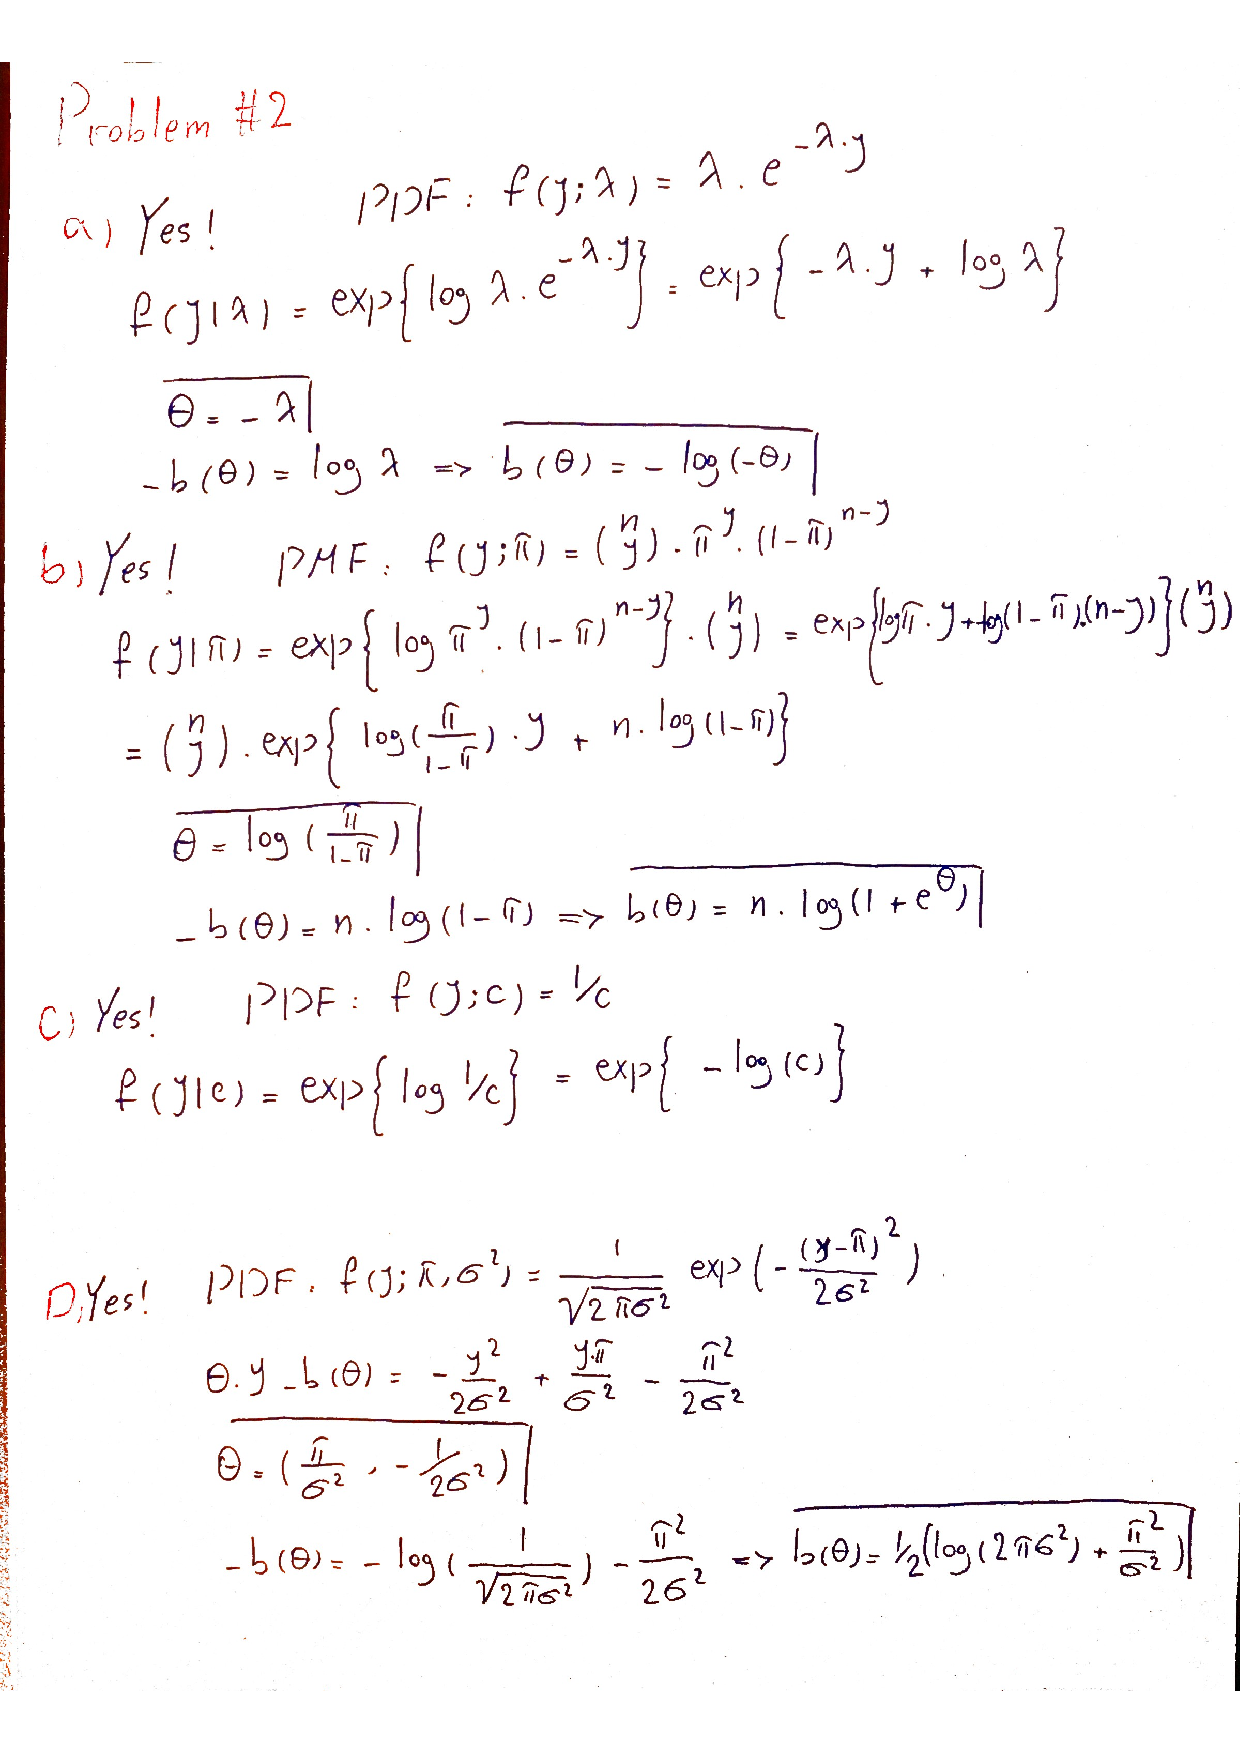
\includepdf[pages=-]{/Users/alimos313/Downloads/day8_problem2.pdf}

\end{document}
